%%%%%%%%%%%%%%%%%%%%%%%%%%%%%%%%%%%%%%%%%%%%%%%%%%%%%%%%%%%%%%%%%%%%%%%%%%%%%%%
%%
%% Copyright © 2022 Tropic Square s.r.o. (https://tropicsquare.com/)
%%
%% This work is subject to the license terms of the LICENSE.txt file in the
%% root directory of this source tree.
%%
%% If a copy of the LICENSE file was not distributed with this work, you can
%% obtain one at (https://tropicsquare.com/license).
%%
%%%%%%%%%%%%%%%%%%%%%%%%%%%%%%%%%%%%%%%%%%%%%%%%%%%%%%%%%%%%%%%%%%%%%%%%%%%%%%%

\documentclass{tropic_design_spec}

% For code samples
\usepackage{listings}
\lstset{backgroundcolor=\color{lightgray}}

%%%%%%%%%%%%%%%%%%%%%%%%%%%%%%%%%%%%%%%%%%%%%%%%%%%%%%%%%%%%%%%%%%%%%%%%%%%%%%%
% Document properties and title page
%%%%%%%%%%%%%%%%%%%%%%%%%%%%%%%%%%%%%%%%%%%%%%%%%%%%%%%%%%%%%%%%%%%%%%%%%%%%%%%
\title{User manual}
\author{Prasoon Dwivedi, Tropic Square}
\date{October 2022}

% Start of document
\begin{document}

% Parameters Needed by Design spec class (must be inside document)
% Set these parameters according to your project.
\def \projectname {Tropic Square Memory Map Generator}
\def \documentname {User manual}
\def \versionnumber {0.2}

% Title page
\maketitle


%%%%%%%%%%%%%%%%%%%%%%%%%%%%%%%%%%%%%%%%%%%%%%%%%%%%%%%%%%%%%%%%%%%%%%%%%%%%%%%
% Document revisions
% We revision with GIT, however, it does not mean that major changes in the
% document should not be kept also with document!
% In general, when you increase document version number, add also entry to
% this table with revisions saying what changed!
%%%%%%%%%%%%%%%%%%%%%%%%%%%%%%%%%%%%%%%%%%%%%%%%%%%%%%%%%%%%%%%%%%%%%%%%%%%%%%%
\section*{Version history}

\begin{TropicRatioLongTable4Col}
    {0.1}            {0.2}                {0.3}            {0.4}
    {Version Tag     & Date                 & Author        &    Description                    }
     0.1             & 18.10.2022           & Prasoon Dwivedi   &    Initial version \Ttlb
     0.2             & 01.11.2022           & Prasoon Dwivedi   &    Add LaTeX output \Ttlb
\end{TropicRatioLongTable4Col}

%%%%%%%%%%%%%%%%%%%%%%%%%%%%%%%%%%%%%%%%%%%%%%%%%%%%%%%%%%%%%%%%%%%%%%%%%%%%%%%
% Table of contents
%%%%%%%%%%%%%%%%%%%%%%%%%%%%%%%%%%%%%%%%%%%%%%%%%%%%%%%%%%%%%%%%%%%%%%%%%%%%%%%
\pagebreak
\tableofcontents
\pagebreak

%%%%%%%%%%%%%%%%%%%%%%%%%%%%%%%%%%%%%%%%%%%%%%%%%%%%%%%%%%%%%%%%%%%%%%%%%%%%%%%
% Introduction
%%%%%%%%%%%%%%%%%%%%%%%%%%%%%%%%%%%%%%%%%%%%%%%%%%%%%%%%%%%%%%%%%%%%%%%%%%%%%%%
\section{Introduction}
This document is a user guide for Tropic Square's memory map generator script (as part of 
the \textit{ts-hw-scripts} repository). This script uses a YAML files containing 
hierarchical memory descriptions to generate:

\begin{itemize}
    % TODO TVE stands for verification not validation
    \item{XML formatted register model used by the Tassic Validation Environment.}
    \item{LaTeX documentation for register models or memory maps.}
\end{itemize}

\subsection*{Distribution model}
The memory map generator is part of \textit{ts-hw-scripts} and is enabled by individual
repositories via their \textit{setup_env} scripts. However it does requires ORDT
(\textit{Open Register Design Tool}) to be enabled with HW scripts.

%%%%%%%%%%%%%%%%%%%%%%%%%%%%%%%%%%%%%%%%%%%%%%%%%%%%%%%%%%%%%%%%%%%%%%%%%%%%%%%
% User manual
%%%%%%%%%%%%%%%%%%%%%%%%%%%%%%%%%%%%%%%%%%%%%%%%%%%%%%%%%%%%%%%%%%%%%%%%%%%%%%%
\pagebreak
\section{User manual}

%%%%%%%%%%%%%%%%%%%%%%%%%%%%%%%%%%%%%%%%%%%%%%%%%%%%%%%%%%%%%%%%%%%%%%%%%%%%%%%
\subsection{Tool setup}
\label{sec:tool-setup}
%%%%%%%%%%%%%%%%%%%%%%%%%%%%%%%%%%%%%%%%%%%%%%%%%%%%%%%%%%%%%%%%%%%%%%%%%%%%%%%

Once \textit{ts-hw-scripts} and \textit{ordt} have been configured via \textit{ts_sw_setup.yml},
they can be verified by running: 
\begin{lstlisting}
which ts_mem_map_generate.py
which ordt_run.sh
\end{lstlisting}
    The command shall output the path like so:
\begin{lstlisting}
/tools/tropic/ts-hw-scripts/v0.18/scripts/ts_mem_map_generate.py
/tools/tropic/ordt/220701.01/ordt_run.sh
\end{lstlisting}

%%%%%%%%%%%%%%%%%%%%%%%%%%%%%%%%%%%%%%%%%%%%%%%%%%%%%%%%%%%%%%%%%%%%%%%%%%%%%%%%%%%%%%%%%
\pagebreak
\subsection{Tool use model}
%%%%%%%%%%%%%%%%%%%%%%%%%%%%%%%%%%%%%%%%%%%%%%%%%%%%%%%%%%%%%%%%%%%%%%%%%%%%%%%%%%%%%%%%%

A basic model used by the memory map generator is shown in the following figure:
\begin{figure}[h]
    \centering
    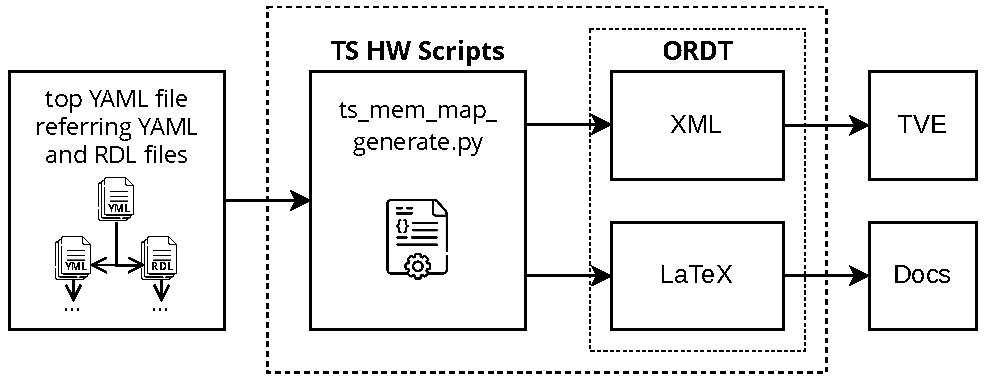
\includegraphics[width=\linewidth]{\detokenize{img/ts_mem_map_main_block_diagram.pdf}}
    \caption{Memory map generator - Use model. }
\end{figure}

%%%%%%%%%%%%%%%%%%%%%%%%%%%%%%%%%%%%%%%%%%%%%%%%%%%%%%%%%%%%%%%%%%%%%%%%%%%%%%%%%%%%%%%%%
\subsection{Input file}
%%%%%%%%%%%%%%%%%%%%%%%%%%%%%%%%%%%%%%%%%%%%%%%%%%%%%%%%%%%%%%%%%%%%%%%%%%%%%%%%%%%%%%%%%
The input YAML file describes the topmost level memory region. It can also refer other YAML
files that follow the same format or RDL files. These YAML files do not define individual 
registers, but memory regions. Using TASSIC as an example memory region, the minimal
required content for every region/subregion is:
\begin{lstlisting}
    name:       TASSIC memory map
    start_addr: 0x00000000
    end_addr:   0xFFFFFFFF
\end{lstlisting}
Every region/subregion may also contain \textbf{either} a \textit{reg_map} or a 
\textit{regions} element, but never both. If a region contains neither key, it 
will be treated as an empty memory space (a region without any registers).
Grammar for all five keywords is discussed in upcoming sections.
\newline
The following section shows an example input file, and more examples can be found in the
\textit{ts-hw-scripts} repository.
%%%%%%%%%%%%%%%%%%%%%%%%%%%%%%%%%%%%%%%%%%%%%%%%%%%%%%%%%%%%%%%%%%%%%%%%%%%%%%%%%%%%%%%%%
\pagebreak
\subsection{Input file example}
\label{ex:input-file-example}
%%%%%%%%%%%%%%%%%%%%%%%%%%%%%%%%%%%%%%%%%%%%%%%%%%%%%%%%%%%%%%%%%%%%%%%%%%%%%%%%%%%%%%%%%
Consider two files like so: \newline
\begin{minipage}{0.475\textwidth}
\begin{lstlisting}
./tassic.yml -> input file

name: TASSIC memory map
start_addr: 0x0000
end_addr: 0xFFFF
regions:
    - name: CPU Sub-System
      start_addr: 0x0000
      end_addr: 0x1FFF
      regions: cpu_ss.yml

    - name: SoC Controller
      start_addr: 0x2000
      end_addr: 0x2FFF
      reg_map: soc_ctrl.rdl
\end{lstlisting}
\end{minipage}%
\hfill
\begin{minipage}{0.475\textwidth}
\begin{lstlisting}
./cpu_ss.yml

name: CPU Sub-System local map
start_addr: 0x0000
end_addr: 0x1FFF
regions:
    - name: Interrupt Controller
      start_addr: 0x0100
      end_addr: 0x01FF
      reg_map: irq_ctrl.rdl

    - name: Timer
      start_addr: 0x0200
      end_addr: 0x02FF
      reg_map: timer.rdl
\end{lstlisting}
\end{minipage}%
\newline
In this example, \textit{tassic.yml} is the only input file. However it references external yaml
and rdl files. It helps to imagine each memory subregion as a node in a generic tree structure.
Each node is a data structure and it can have an arbitrary number of children nodes. Figure
\ref{fig:hierarchy-tree} shows the above example visualised as a generic tree.
\pagebreak
\begin{figure}[h]
    \centering
    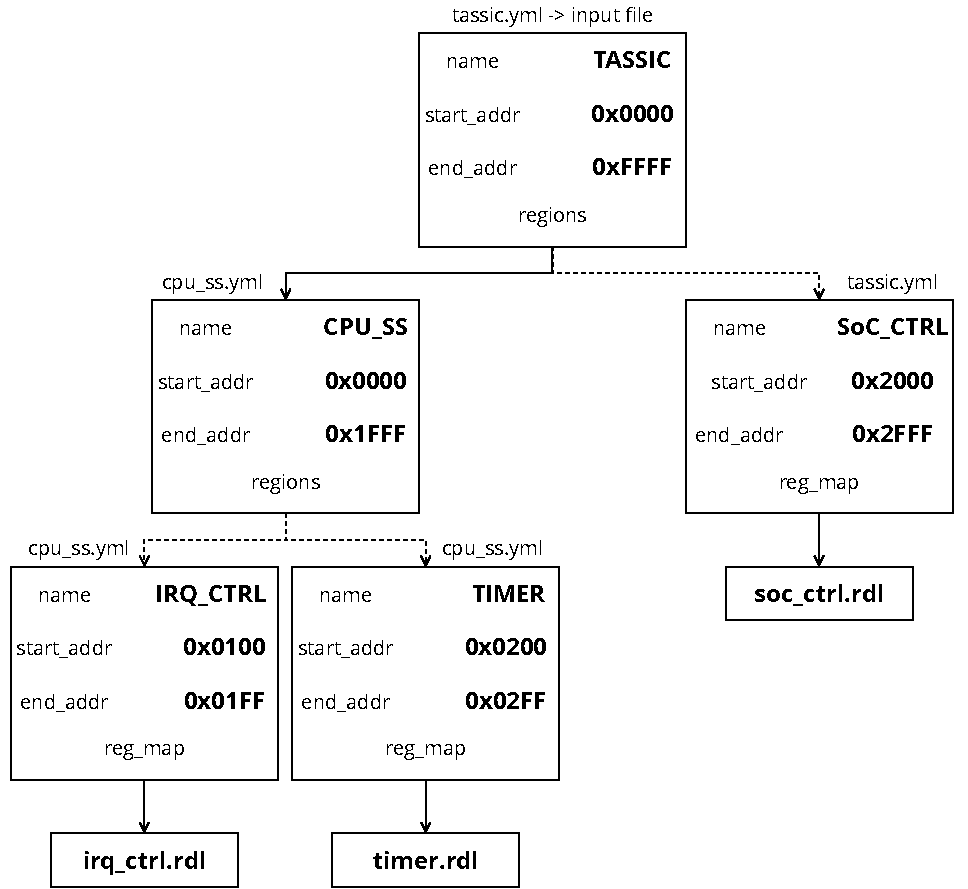
\includegraphics[width=\linewidth]{\detokenize{img/ts_mem_map_hierarchy_diagram.pdf}}
    \caption{Input file hierarchical structure.}
    \label{fig:hierarchy-tree}
\end{figure}

In figure \ref{fig:hierarchy-tree}, solid lines represent an external file being referenced
and dashed lines represent new subregions being read from the same file. 

%%%%%%%%%%%%%%%%%%%%%%%%%%%%%%%%%%%%%%%%%%%%%%%%%%%%%%%%%%%%%%%%%%%%%%%%%%%%%%%%%%%%%%%%%
\pagebreak
\subsection{Grammar for keyword \textit{name}}
%%%%%%%%%%%%%%%%%%%%%%%%%%%%%%%%%%%%%%%%%%%%%%%%%%%%%%%%%%%%%%%%%%%%%%%%%%%%%%%%%%%%%%%%%

Since the name is fed to ORDT as a hardware block name and eventually to a LaTeX compiler,
it can not be a SystemRDL or LaTeX keyword. Any brackets in the name will also be replaced 
with underscores by the script.

%%%%%%%%%%%%%%%%%%%%%%%%%%%%%%%%%%%%%%%%%%%%%%%%%%%%%%%%%%%%%%%%%%%%%%%%%%%%%%%%%%%%%%%%%
\subsection{Grammar for keywords \textit{start_addr} and \textit{end_addr}}
%%%%%%%%%%%%%%%%%%%%%%%%%%%%%%%%%%%%%%%%%%%%%%%%%%%%%%%%%%%%%%%%%%%%%%%%%%%%%%%%%%%%%%%%%

The start and end addresses need to be offsets relative to their parent block.
For example, consider a block and a sub-block like so:
\begin{lstlisting}
name:       My example block
start_addr: 0x1000
end_addr:   0xFFFF
regions:
    - name:       My example Sub-block
      start_addr: 0x10
      end_addr:   0x1F
      reg_map:    foo.rdl
\end{lstlisting}
The script will sum up these offsets and write absolute addresses to the output.
This summing up of address offsets is done for all levels of nesting; and
since a block can refer an RDL file, the address offsets of those registers are also
summed up to write the absolute address to the output. \newline
If \textit{foo.rdl} from the above example were to define a register \textit{r_foo}
at offset 0x04, then the output would list the base address of \textit{r_foo} as 0x1014.
\newline
Using the \textit{--lint} switch, you can also ask the script to reject subregions
with address ranges out of bounds of their parent regions. For example, if in the above
code block, \textit{My example Sub-block} had start address \textit{0x10000}, it would be
out of bounds of \textit{My example block}'s address range and would throw an error.

%%%%%%%%%%%%%%%%%%%%%%%%%%%%%%%%%%%%%%%%%%%%%%%%%%%%%%%%%%%%%%%%%%%%%%%%%%%%%%%%%%%%%%%%%
\pagebreak
\subsection{Grammar for keyword \textit{reg_map}}
%%%%%%%%%%%%%%%%%%%%%%%%%%%%%%%%%%%%%%%%%%%%%%%%%%%%%%%%%%%%%%%%%%%%%%%%%%%%%%%%%%%%%%%%%
The \textit{reg_map} keyword lets you refer an RDL file that contains register definitions
of the calling block. When a block calls an RDL file, it can not contain any sub blocks
because the RDL file already contains everything within the calling block.
\newline
Please keep in mind the distinction between definitions of registers and subregions.
The input and referenced yaml files used by this script do not define individual registers;
they describe regions that contain registers and therefore lie an abstraction level
above RDL files.
\newline
For example, in the below snippet, \textit{timer.rdl} contains the actual register definitions
for the \textit{Timer 1} sub-block.

\begin{lstlisting}
name:       CPU Sub-system
start_addr: 0x00000000
end_addr:   0x01FFFFFF
regions:
    - name:       Timer 1
      start_addr: 0x01100000
      end_addr:   0x01100FFF
      reg_map:    timer.rdl
\end{lstlisting}

The path to an RDL file must be relative to the file that calls it. You may also use general
filesystem identifiers like '..' to indicate a parent derectory.

%%%%%%%%%%%%%%%%%%%%%%%%%%%%%%%%%%%%%%%%%%%%%%%%%%%%%%%%%%%%%%%%%%%%%%%%%%%%%%%%%%%%%%%%%
\pagebreak
\subsection{Grammar for keyword \textit{regions}}
%%%%%%%%%%%%%%%%%%%%%%%%%%%%%%%%%%%%%%%%%%%%%%%%%%%%%%%%%%%%%%%%%%%%%%%%%%%%%%%%%%%%%%%%%
The \textit{regions} keyword lets you define a nested set of sub-blocks either within the
same file, or by referencing an external YAML file of the same format. Consider the following 
example:

\begin{lstlisting}
name:       TASSIC memory map
start_addr: 0x00000000
end_addr:   0xFFFFFFFF
regions:
    - name:       CPU Sub-System
      start_addr: 0x0000000
      end_addr:   0x1FFFFFF
      regions:
          - name:       Timer 1
            start_addr: 0x1100000
            end_addr:   0x1100FFF
            reg_map:    timer.rdl

          - name:       Timer 2
            start_addr: 0x1200000
            end_addr:   0x1200FFF
            reg_map:    timer.rdl
\end{lstlisting}

In the above snippet, both regions \textit{Timer 1} and \textit{Timer 2} could be described
in an external YAML file like so:

\begin{lstlisting}
name:       TASSIC memory map
start_addr: 0x00000000
end_addr:   0xFFFFFFFF
regions:
    - name:       CPU Sub-System
      start_addr: 0x00000000
      end_addr:   0x01FFFFFF
      regions:    cpu_ss.yml
\end{lstlisting}

This included YAML file follows the same format and grammars. Paths to external files being
referenced are relative to the files referencing them. These external files can also reference
more files. \textit{ts_mem_map_generate.py} supports up to 5 nested YAML files describing
hierarchical memory maps. If the maximum number of nested files is exceeded, the script
will throw an error.

%%%%%%%%%%%%%%%%%%%%%%%%%%%%%%%%%%%%%%%%%%%%%%%%%%%%%%%%%%%%%%%%%%%%%%%%%%%%%%%%%%%%%%%%%
\pagebreak
\subsection{Notes}
%%%%%%%%%%%%%%%%%%%%%%%%%%%%%%%%%%%%%%%%%%%%%%%%%%%%%%%%%%%%%%%%%%%%%%%%%%%%%%%%%%%%%%%%%

\begin{enumerate}
    
    \item{All files being referenced are relative to the file referencing them.}

    \item{Consider the example from Section \ref{ex:input-file-example}. Notice how 
    \textit{CPU Sub-System} is defined twice: once in the top level file and again in
    its block level file. When the generator notices this duplicacy, it overwrites the 
    block level definitions with the top level definitions. }

\end{enumerate}

\end{document}
